
\section*{Ejercicios}
\addcontentsline{toc}{section}{\textit{Ejercicios}}



%---------------------------
% Ejercicio 1   
%---------------------------
\begin{Enunciado}
	\subsection*{Ejercicio 1}
	%\addcontentsline{toc}{subsection}{\textit{Ejercicio 1}}

	Indicar la condición de polarización y dibujar los diagramas de bandas de enerǵia y densidad de carga para un MOS ideal de silicio en las isugientes condiciones:

	\begin{enumerate}[label=\alph*)]
		\item $\phi_B= \SI{0.312}{V}$  y  $\phi_S= \SI{0.312}{V}$.
		\item $\phi_B= -\SI{0.234}{V}$  y  $\phi_S= \SI{0.078}{V}$.
		\item $\phi_B= -\SI{0.234}{V}$  y  $\phi_S= -\SI{0.468}{V}$.
		\item $\phi_B= \SI{0.390}{V}$  y  $\phi_S= \SI{0.936}{V}$.
	\end{enumerate}
\end{Enunciado}

\vspace*{1em}

Indicar la condición de polarización es indicar básicamente si está en acumulación $(\phi_S<0)$, en plana $(\phi_S=0)$, en vaciamiento $(\phi_S>0$) o en inversa $(\phi_S>2\phi_F$).

Por definición los valores de $\phi_B$ y $\phi_S$ son:

\begin{equation*}
	\phi_F \equiv \phi_B \equiv E_i(\text{sustrato}) - E_F \tquad
	\phi_S \equiv E_i(\text{sustrato}) - E_i (\text{interfaz})
\end{equation*}
Por lo tanto, para determinar el tipo de semiconductor debemos usar, debemos observar el signo de $\phi_B$. Si $\phi_B > 0$, el semiconductor es de tipo p, y si $\phi_B < 0$, el semiconductor es de tipo n. Esto se debe a que $\phi_B$ está relacionado con la posición del nivel de Fermi respecto al nivel intrínseco.
\begin{itemize}
	\item Si $\phi_B > 0$, el nivel de Fermi está por debajo del nivel intrínseco, indicando un semiconductor tipo p.
	\item Si $\phi_B < 0$, el nivel de Fermi está por encima del nivel intrínseco, indicando un semiconductor tipo n.
\end{itemize}
Con esta información, podemos determinar tanto la condición de polarización como el tipo de semiconductor para cada caso. Esto será importante ya que nos dirá que carga en la interfaz (si la del metal o la del semiconductor) es postiiva o negativa.


\begin{enumerate}[label=\alph*)]
	\item Estamos ante un semiconductor tipo $P$, en la región de vaciamiento o intrínseco (ya que $\phi_S =  \phi_F$).
	      \begin{figure}[H]\centering
		      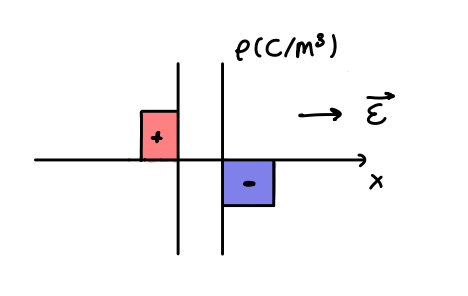
\includegraphics[width=0.45\linewidth]{Ejercicios/Ch_05/Ej_01_a1.png} \hfill
		      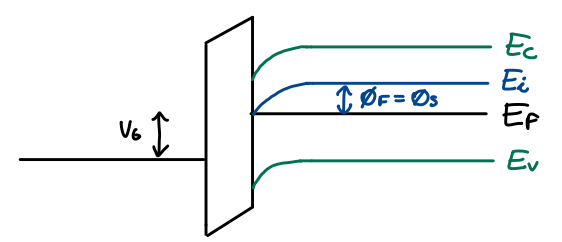
\includegraphics[width=0.45\linewidth]{Ejercicios/Ch_05/Ej_01_a2.png}
	      \end{figure}
	\item Estamos ante un semiconductor tipo $N$ en la región de acumulación.
	      \begin{figure}[H]\centering
		      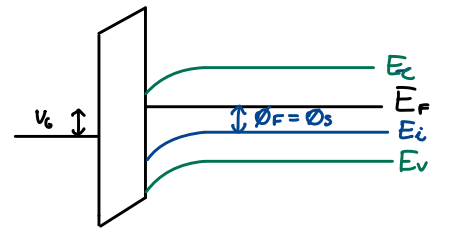
\includegraphics[width=0.45\linewidth]{Ejercicios/Ch_05/Ej_01_b1.png} \hfill
		      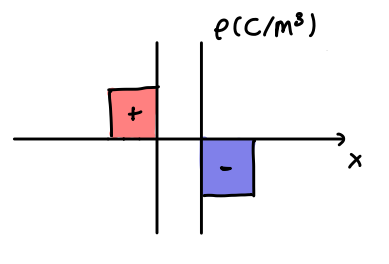
\includegraphics[width=0.45\linewidth]{Ejercicios/Ch_05/Ej_01_b2.png}
	      \end{figure}
	\item Estamos ante un semiconductor tipo $N$ en la región de transición entre vaciamiento e inversión ($\phi_S=2\phi_F$).

	      \begin{figure}[H]\centering
		      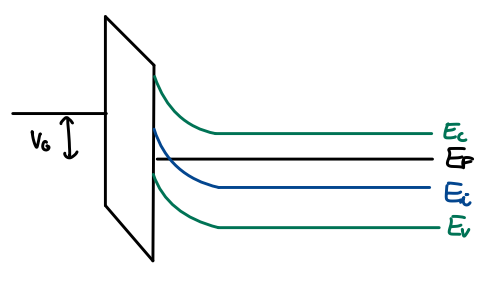
\includegraphics[width=0.45\linewidth]{Ejercicios/Ch_05/Ej_01_c1.png} \hfill
		      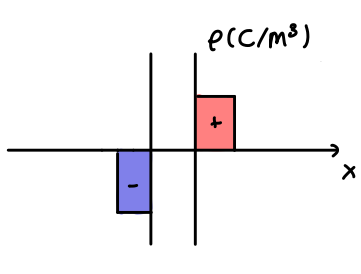
\includegraphics[width=0.45\linewidth]{Ejercicios/Ch_05/Ej_01_c2.png}
	      \end{figure}
	\item Estamos ante un semiconductor tipo $P$ en la región de inversión.

	      \begin{figure}[H]\centering
		      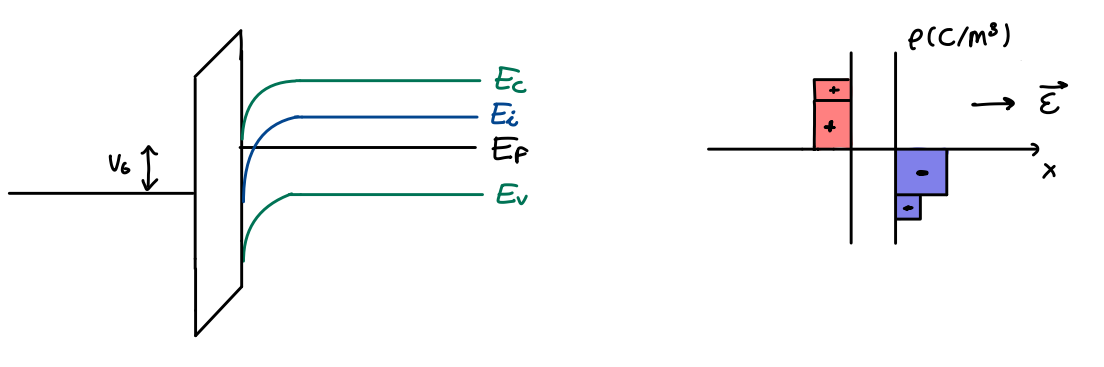
\includegraphics[width=0.9\linewidth]{Ejercicios/Ch_05/Ej_01_d.png}
	      \end{figure}
\end{enumerate}

\vspace*{2em}

%---------------------------
% Ejercicio 2
%---------------------------

\begin{Enunciado}
	\subsection*{Ejercicio 2}
	%\addcontentsline{toc}{subsection}{\textit{Ejercicio 2}}
	Un MOS ideal se mantiene constante a una temperatura $T=300$ K con $x_0=\SI{0.1}{\mu m}$ con un dopado del Si de $N_A=\SI{1e15}{cm^{-3}}$ (la constante dieléctrica relativa para el óxido es de 3.9). Calcula y representa:
	\begin{enumerate}[label=\alph*)]
		\item $\phi_B \equiv \phi_F$ y la anchura de la región de vaciamiento cuando $\phi_B = \phi_S$
		\item El campo eléctrico y la tensión aplicada en la puerta cuando $\phi_B = \psi_S$.
	\end{enumerate}
\end{Enunciado}

\vspace*{1em}

Las soluciones son, por apartado:

\begin{enumerate}[label=\alph*)]
	\item Conociendo $N_A$ y que $T=300$K podemos obtner $\phi_B = \phi_F$ ($n_i \approx \SI{1e10}{cm^{-3}}$ a 300 K). Luego como concemos $\phi_S$ en virtud de $\phi_B = \phi_S$, el cálculo de la anchura será trivial ya qie la solo depende de $\phi_S$.

	      \begin{equation*}
		      \phi_S = \phi_F = \frac{1}{q} \parentesis{E_i(\text{sustrato})-E_F} = \frac{kT}{q} \log \parentesis{\frac{N_A}{n_i}} \qquad
		      \phi_{S} = \SI{2.98e-01}{V}
	      \end{equation*}
	      tal que

	      \begin{equation*}
		      W = \sqrt{\frac{2\phi_S K_S \epsilon_0}{qN_A}} \qquad
		      W = \SI{6.24e-05}{cm}
	      \end{equation*}

	\item El campo elećtrico también se puede calcular facilmente, ya que en la zona S solo depende de $W$ (y de $N_A$ y $K_{S}$) y en la zona O depende de $\Ecal_{sc}$ en la interfaz y de las permitividades relativas. Al suponer metal perfecto no hay campo elećtrico en el metal. Veamos que:

	      \begin{equation*}
		      \Ecal_S (x) = \left\lbrace \begin{array}{ll}
			      \frac{qN_A}{K_S \epsilon_0} (W-x) & \quad \text{si} \ 0\leq x \leq W \\
			      0                                 & \quad \text{si} \ W<x
		      \end{array} \right.
	      \end{equation*}
	      Luego la tensión aplicada también la podemos calcular facilmente a través de las fórmulas:

	      \begin{equation*}
		      V_G = \phi_S + \frac{K_S}{K_o} x_o \sqrt{\frac{2qN_A}{K_S\epsilon_0} \phi_s}
	      \end{equation*}
	      Las soluciones son:

	      \begin{equation*}
		      \Ecal(0) = \SI{6.96e+03}{V/cm} \qquad
		      V_G = \SI{5.85e-01}{V}
	      \end{equation*}

	      	\begin{figure}[H]\centering
		      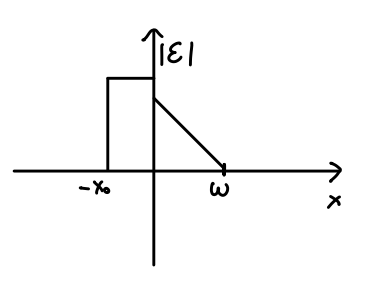
\includegraphics[width=0.45\linewidth]{Ejercicios/Ch_05/Ej_02_a.png} \hfill
		      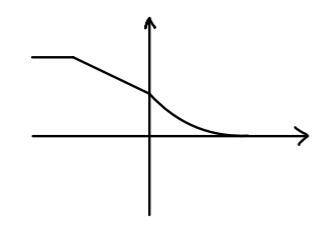
\includegraphics[width=0.45\linewidth]{Ejercicios/Ch_05/Ej_02_c.png}
			\centering\end{figure}

			Aunque no nos lo piden, las bandas dibujadas:
			\begin{figure}[H]\centering
				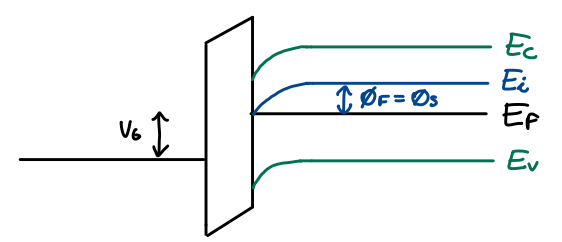
\includegraphics[width=0.45\linewidth]{Ejercicios/Ch_05/Ej_02_b.png}
			  \centering\end{figure}
  

\end{enumerate}



\vspace*{2em}

%---------------------------
% Ejercicio 3
%---------------------------

\begin{Enunciado}
	\subsection*{Ejercicio 3}
	%\addcontentsline{toc}{subsection}{\textit{Ejercicio 3}}
	Dibujar la distribución de carga, de campo eléctrico y de potencial en un MOS ideal con sustrato tipo N bajo condiciones de acumulación, vaciamiento e inversión (incluir en la representación las tres zonas que componen el dispositivo: metal, óxido y semiconductor). Considerando una puerta de polisilicio de tipo N, un espesor de óxido de silicio de 50 nm con constante dieléctrica relativa par el óxido de 3.9 y con un dopado de $N_D = \SI{5.0e16}{cm^{-3}}$, calcula:
	\begin{enumerate}[label=\alph*)]
		\item Capacidad del óxido. 
		\item Tensión de banda plana.
		\item Tensión umbral ideal.
		\item Tensión umbral real. 
	\end{enumerate}
\end{Enunciado}

\vspace*{1em}

	En primer lugar nos mandan dibujar las gráficas de: distribución de carga, campo eléctrico y potencial en el MOS ideal de sustrato N para los 3 casos típicos: acumulación, vaciamiento e inversión. Así pues: 
	\begin{itemize}
		\item Acumulación:
		\begin{figure}[H]\centering
			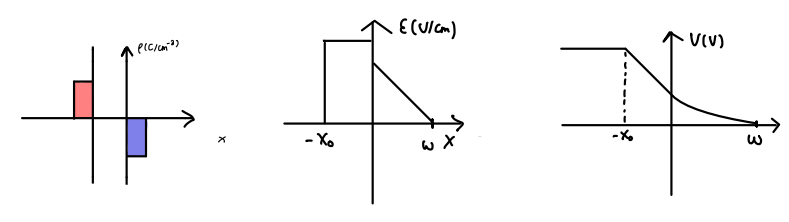
\includegraphics[width=0.8\linewidth]{Ejercicios/Ch_05/Ej_03_a1.png}
		\end{figure}
		\item Vaciamiento:
		\begin{figure}[H]\centering
			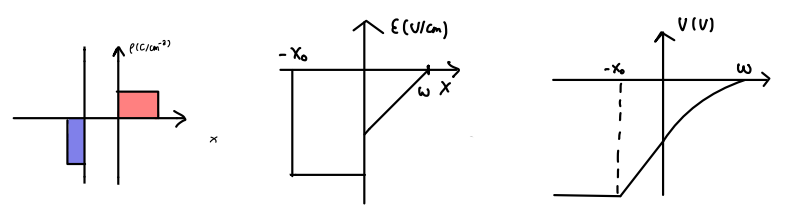
\includegraphics[width=0.8\linewidth]{Ejercicios/Ch_05/Ej_03_a2.png}
		\end{figure}
		\item Inversión:
		\begin{figure}[H]\centering
			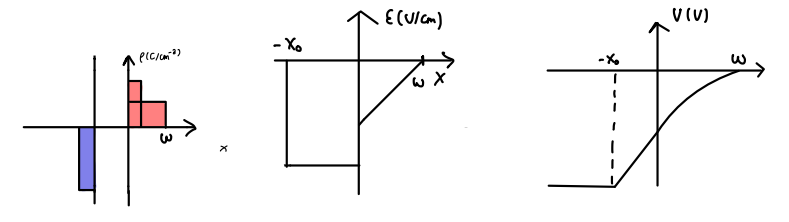
\includegraphics[width=0.8\linewidth]{Ejercicios/Ch_05/Ej_03_a3.png}
		\end{figure}
	\end{itemize}


\begin{enumerate}[label=\alph*)]
	\item Para calcular la capacidad del óxido solo tenemos que hacer: 
\end{enumerate}


%---------------------------
% Ejercicio 4
%---------------------------

\begin{Enunciado}
	\subsection*{Ejercicio 4}
	%\addcontentsline{toc}{subsection}{\textit{Ejercicio 4}}

	Para un dispositivo MOS SiO$_2$-Si ideal con espesor de óxiddo de 5 nm, $N_A = \SI{1e17}{cm^{-3}}$ y una constante dieléctrica relativa para el óxido de 3.9, calcula y representa la tensión de puerta y el campo elećtrico de la interfaz necesarios para que el Silicio en la interfaz se comporte como un intrínseco.
\end{Enunciado}

Recordamos que para que el silicio en la interfaz se comporte como un intrínseco debe verificarse que:

\begin{equation*}
	E_i(\text{interfaz}) - E_F = 0
\end{equation*}
es decir, que:

\begin{equation*}
	\phi_S = \phi_F \qquad
	\phi_{S} = \SI{4.17e-01}{V}
\end{equation*}
ya que

\begin{equation*}
	\phi_F \equiv \phi_B \equiv E_i(\text{sustrato}) - E_F \tquad
	\phi_S \equiv E_i(\text{sustrato}) - E_i (\text{interfaz})
\end{equation*}
Entonceses trivial el cálculo de la tensión de puerta $V_G$ y $\Ecal(\text{interfaz})$, ya que es simplemente aplicar las ecuaciones:

\begin{equation*}
	W = \sqrt{\frac{\phi_S K_S \epsilon_0}{qN_A}}
\end{equation*}
\begin{equation*}
	\Ecal_S (\text{interfaz}) = \frac{qN_A}{K_S \epsilon_0}W
\end{equation*}
\begin{equation*}
	V_G = \phi_S + \frac{K_S}{K_o} x_o \sqrt{\frac{2qN_A}{K_S\epsilon_0} \phi_s}
\end{equation*}
Así pues:

\begin{equation*}
	W = \SI{7.34e-06}{cm} \quad
	E(0) = \SI{1.14e+05}{V/cm} \quad 
	V_G = \SI{5.87e-01}{V}
\end{equation*}
\begin{figure}[H] \centering
	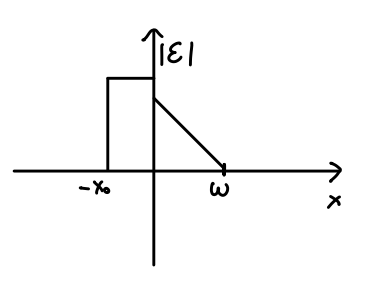
\includegraphics[width=0.45\linewidth]{Ejercicios/Ch_05/Ej_04_a.png} \hfill
	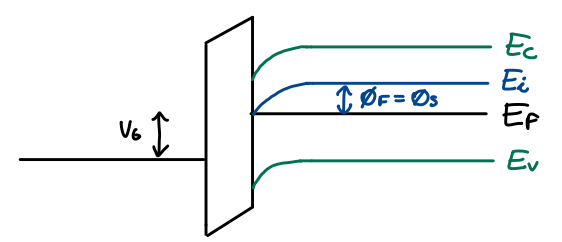
\includegraphics[width=0.45\linewidth]{Ejercicios/Ch_05/Ej_04_b.png}
\end{figure}

\vspace*{2em}
%---------------------------
% Ejercicio 5
%---------------------------

\begin{Enunciado}
	\subsection*{Ejercicio 5}
	%\addcontentsline{toc}{subsection}{\textit{Ejercicio 5}}
	La concentración de electrones en los contactos de fuente y drenador de un MOSFET de silicio es de $\SI{1e+17}{cm^{-3}}$, y la tensión aplicada bajo la puerta hace que la concetración de electroens sea de $\SI{1e+9}{cm^{-3}}$. Si suponemos que la corriente qeu fluye es despreciable, calcula y representa la barrera que ven los portadores. 
\end{Enunciado}

\vspace*{1em}

	Como sabemos, $n=\SI{1e+9}{cm^{-3}}$ es menor que $n_i =\SI{1e+10}{cm^{-3}}$, por lo que la región entre fuente y drenador es de tipo P. Teniendo en cuenta que nos dicen que la corriente es despreciable, esto es, el nivel de Fermi es constante, podemos hacer un dibujo de las bandas, aunque de manera esquemática (recordemos que en realidad en la zona de vaciamiento se curvan,  no son líneas rectas):

\begin{figure}[H] \centering
	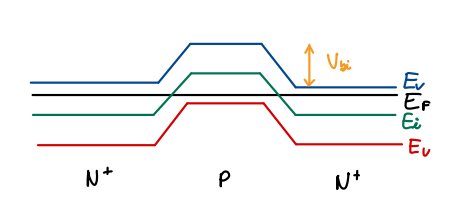
\includegraphics[width=0.45\linewidth]{Ejercicios/Ch_05/Ej_05.png} \hfill
\end{figure}

	De lo que se puede deducir que el salto $\Vbi$ es:

	\begin{equation}
		E_i|_P - E_i|_{N^+} =  - kT \log \parentesis{\frac{n_P}{n_i}} - kT  \log \parentesis{\frac{n_N}{n_i}}  = 0.059264 + 0.41668 \ \eV = 0.4789 \ \eV 
	\end{equation}


\vspace*{2em}

%---------------------------
% Ejercicio 6
%---------------------------

\begin{Enunciado}
	\subsection*{Ejercicio 6}
	%\addcontentsline{toc}{subsection}{\textit{Ejercicio 6}}
	Para un MOSFET con puerta de polisilicio tipo N y canal tipo n de silicio con un espesor de la capa de óxido de 50 nm, $N_A = \SI{5e16}{cm^{-3}}$, $\epsilon_{ox}=3.9$, $\epsilon_{Si} = 11.9$ y $\chi=4.05 \eV$, calcular:
	\begin{enumerate}[label=\alph*)]
		\item Capacidad del óxido, la tensión de la anda plana y la tensión umbral.
		\item Representa las bandas en equilibrio térmico.
		\item Representa la estructura de bandas y la densidad de carga cuando el MOS está en inversión, vaciamiento y en acumulación.
	\end{enumerate}
\end{Enunciado}

\vspace*{1em}
La solución es:
\begin{enumerate}[label=\alph*)]
	\item El valor de la capacidad del óxido viene dado por la siguiente ecuación:
	      \begin{equation*}
		      \frac{C}{A} = \frac{\epsilon_0 K_{ox}}{x_0} = \SI{6.9e-8}{F/cm^{2}}
	      \end{equation*}
	      y los valores de la tensión de banda plana viene dada por

	      \begin{equation*}
		      qV_{FB} = q\phi_{ms} = q(\phi_m - \phi_s) = q\phi_m -  \parentesis{\chi + E_c - E_F} = q \chi - q \chi -  \parentesis{E_c  - E_F}
	      \end{equation*}
	      que podmeos simplificar como:
	      \begin{equation*}
		      qV_{FB} =  (E_c - E_F) = (E_c - E_i) + (E_i - E_f) = \frac{E_g}{2} + q\phi_B
	      \end{equation*}
	      tal que si
	      \begin{equation*}
		      \phi_B = \frac{kT}{q} \ln \parentesis{N_A/n_i} = \SI{0.4}{V}
	      \end{equation*}
	      y por tanto la \textbf{la tensión de banda plana} es

	      \begin{equation*}
		      V_{FB} = -\SI{0.961}{V}
	      \end{equation*}
	      Y \textbf{la tensión umbral} es

	      \begin{equation*}
		      V_T = \varphi_B + \frac{K_S}{K_{ox}}  x_0 \sqrt{\frac{2q N_A \psi_B}{K_S \epsilon_0}}  = \SI{2.48}{V}
	      \end{equation*}
	      Todo esto ha sido idealmente.
	\item Representa las bandas en equilibrio térmico.
	\item Representa la estructura de bandas y la densidad de carga cuando el MOS está en inversión, vaciamiento y en acumulación.
\end{enumerate}


\vspace*{2em}

%---------------------------
% Ejercicio 7
%---------------------------
\begin{Enunciado}
	\subsection*{Ejercicio 7}
	%\addcontentsline{toc}{subsection}{\textit{Ejercicio 7}}
	Para un MOSFET con puerta de aluminio (4.08 eV) y canal tipo n de silicio con un espesor de la capa de óxido de 30 nm, $N_A = \SI{1e16}{cm^{-3}}$ con $Q_F/q=\SI{1e10}{cm^{-2}}$, $\epsilon_{ox}=3.9$, $\chi_{ox}=1.1 \eV$, $Eg_{ox}=8.9$ eV, $\epsilon_{Si} = 11.9$ y $\chi_{Si}=4.05 \eV$, calcular:
	\begin{enumerate}[label=\alph*)]
		\item Capacidad del óxido, la tensión de la anda plana y la tensión umbral.
		\item Representa las bandas en equilibrio térmico.
		\item Representa la estructura de bandas y la densidad de carga cuando el MOS está en los otros casos de polarización posibles.
	\end{enumerate}
\end{Enunciado}
\vspace*{1em}
Solucion:
\begin{enumerate}[label=\alph*)]
	\item La capacidad del óxido viene dada por:
	\begin{equation*}
		\frac{C_{ox}}{A} = \frac{\epsilon_0 K_{ox}}{x_0} = \SI{1.15e-7}{F/cm^{2}}
	\end{equation*}
	y los valores de la tensión de banda plana viene dada por

	\begin{equation*}
		qV_{FB} = q\phi_{ms} = q(\phi_m - \phi_s) = q\phi_m -  \parentesis{\chi + E_c - E_F} = q \chi - q \chi -  \parentesis{E_c  - E_F}
	\end{equation*}
	que podmeos simplificar como:
	\begin{equation*}
		qV_{FB} =  (E_c - E_F) = (E_c - E_i) + (E_i - E_f) = \frac{E_g}{2} + q\phi_B
	\end{equation*}
	tal que si
	\begin{equation*}
		\phi_B = \frac{kT}{q} \ln \parentesis{N_A/n_i} = \SI{0.912e+0}{V}
	\end{equation*}
	y por tanto la \textbf{la tensión de banda plana} es

	\begin{equation*}
	\end{equation*}
	Y \textbf{la tensión umbral} es

	\begin{equation*}
		V_T = 2\varphi_F + \frac{K_S}{K_{ox}}  x_0 \sqrt{\frac{4q N_A \psi_F}{K_S \epsilon_0}}  = \SI{1.14}{V}
	\end{equation*}
	Ahora la real:
	\begin{equation*}
		(V_T)_{real} =(V_T)_{ideal} + V_{FB} = \SI{0.24}{V}
	\end{equation*}
	\item Representa las bandas en equilibrio térmico.
	\item Representa la estructura de bandas y la densidad de carga cuando el MOS está en inversión, vaciamiento y en acumulación.
\end{enumerate}
\vspace*{2em}

%---------------------------
% Ejercicio 8
%---------------------------
\begin{Enunciado}
	\subsection*{Ejercicio 8}
	%\addcontentsline{toc}{subsection}{\textit{Ejercicio 8}}

	\lipsum[1].
\end{Enunciado}
\vspace*{1em}
\lipsum[1].
\vspace*{2em}
%---------------------------
% Ejercicio 9
%---------------------------
\begin{Enunciado}
	\subsection*{Ejercicio 9}
	%\addcontentsline{toc}{subsection}{\textit{Ejercicio 9}}

	\lipsum[1].
\end{Enunciado}
\vspace*{1em}
\lipsum[1].


